\chapter{Machine learning methodology}
\label{ch.ml}

In this chapter, we discuss the machine learning methodology we utilize for our $D^0$ analysis. In Ch. \ref{sec.ml_bdt}, we introduce the theory of boosted decision trees (BDTs), the particular type of model used in this analysis. Then in Ch. \ref{sec.ml_implementation}, we discuss various aspects to consider when applying BDTs and interpreting the results.

% \section{Introduction to machine learning (ML)}
% \label{sec.ml_intro}

% {\color{brown}\bf Resources:}
% BDTs for high energy physics: \cite{BDT}

% \begin{itemize}
%     \item Example of fitting data
%     \item Features, output, and loss function
%     \item Gradient descent
%     \item Regression and classification
%     \item Training, validation, and application
%     \item Overfitting and underfitting
% \end{itemize}

% At its core, machine learning (ML) is about fitting data. As with any statistical analysis, our goal is to identify patterns in a given sample that can be generalized and used to make predictions on new data. 

% %-----------------------------
% \subsection{Machine learning as linear regression}

% %-----------------------------
% \subsection{Gradient descent}

% %-----------------------------
% \subsection{Types of ML models}

% %-----------------------------
% \subsection{Training, validation, and application}

%--------------------------------------------------------
\section{The boosted decision tree (BDT) model}
\label{sec.ml_bdt}


%-----------------------------
\subsection{Decision tree classifiers}

\begin{figure}[h!]
    \centering
    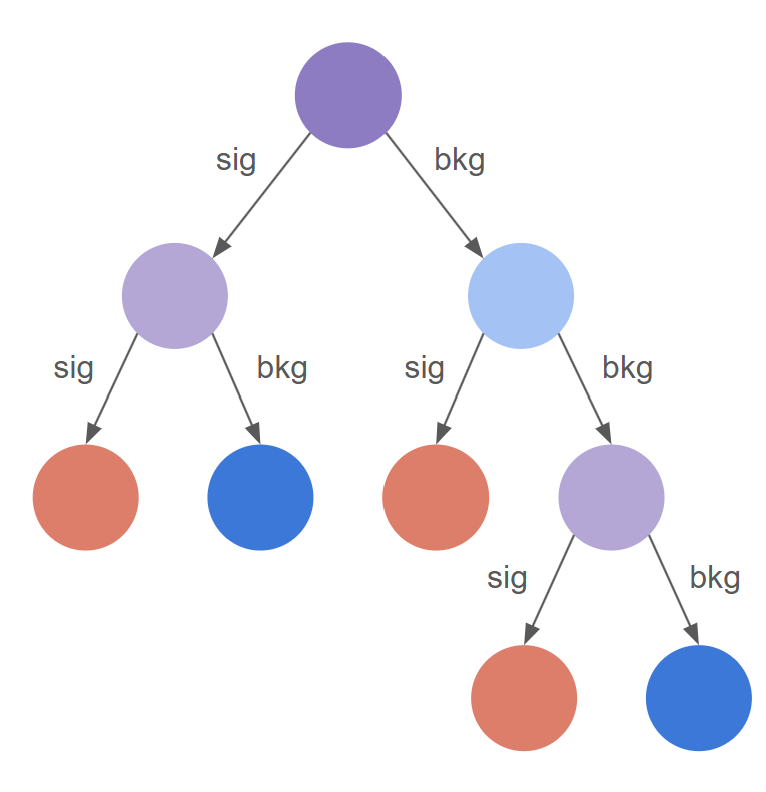
\includegraphics[width=0.4\linewidth]{gallery/ML/decision_tree.png}
    \caption{A decision tree model.}
    \label{f.decision_tree}
\end{figure}
%

A decision tree is a type of machine learning model that classifies data into discrete categories (or classes) by iteratively applying selections on the data features. In this analysis, the data consists of all the reconstructed $D^0$ and background candidates, and the two classes are $D^0$ signal and background. (This is a {\it binary} classification problem, which only involves two classes. In general, decision trees can also be used to separate data into three or more classes.) The features of the data are the topological variables discussed in Ch. \ref{sec:def_top_vars}.

Fig. \ref{f.decision_tree} provides a schematic of a decision tree model. All of the data starts in the top node, known as the root node. The algorithm tries to separate the data into signal and background classes by testing cuts on every possible topological variable, then selects the optimal cut which results in the cleanest separation. According to this topological cut, the data is split into two subsequent child nodes. At each subsequent node, the algorithm repeats the same steps to continue separating the data. When some termination condition is achieved at a given node, that node is prevented from splitting and becomes a leaf node. Common termination conditions include reaching a minimum number of candidates (node size), or achieving a minimum or maximum purity $p$, a value that represents the percentage of signal or background candidates in the node \cite{BDT}. Through this process, the decision tree learns the shape of the multi-dimensional boundaries between signal and background candidates, with respect to the topological features.

When the tree stops splitting, training of the model is complete. In the end, every candidate will have been sorted into one of the signal or background leaf nodes. Each candidate is assigned a prediction, a value representing the likelihood of the candidate being a true signal or background. Depending on the model implementation, this prediction can be a continuous quantity, such as a probability, or a discrete value, such as +1 for belonging to a signal leaf node and 0 (or -1) for belonging to a background leaf node.

Decision trees are structurally simple and functionally intuitive, making them a desirable tool for solving optimization problems in physics. However, they are prone to overfitting and are often unstable, meaning that small changes in the training data can dramatically alter the model structure \cite{BDT}. To offer some insight into this issue, consider the following hypothetical. In order to achieve the cleanest separation of signal and background data, we will most likely want the tree to continue growing until the nodes achieve a very high purity. This will result in a deep tree with many splittings. However, by attempting to perfectly classify all events, the tree becomes sensitive to outliers and noise in the data, memorizing details that are unique to the training data rather than learning general patterns. On the other hand, adopting weak purity requirements to constrain the tree depth can also limit the model's ability to discriminate between signal and background data, still resulting in poor performance.

This is an illustration of the {\it bias-variance tradeoff} in machine learning, in which reducing the rate of incorrect model output (bias) tends to increase model sensitivity to fluctuations in the training data (variance) \cite{BDT}. Often, high bias leads to underfitting while high variance leads to overfitting. Increasing complexity, such as by increasing the depth of a decision tree, tends to tip the model toward high variance. The challenge then is to balance bias and variance in order to both achieve high discriminative ability and mitigate the tendency of overfitting. This is where {\it boosting} comes in.

%-----------------------------
\subsection{Gradient boosting}
\label{sec.ml_gradient_boosting}

%
\begin{figure}[h!]
    \centering
    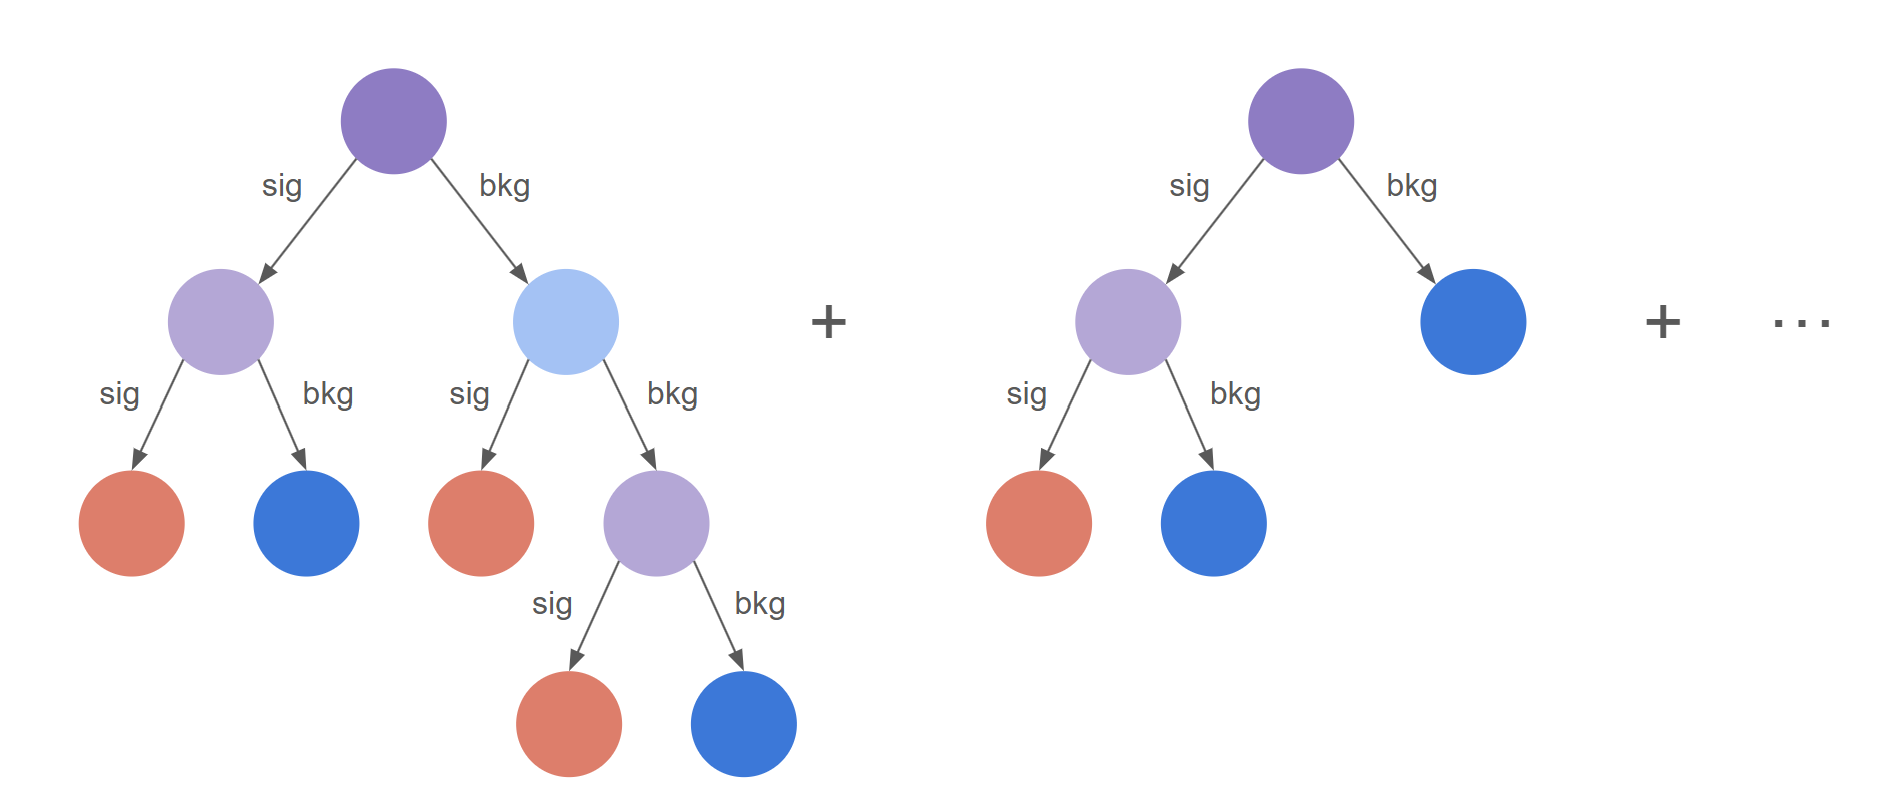
\includegraphics[width=0.9\linewidth]{gallery/ML/boosted_decision_tree.png}
    \caption{A boosted decision tree model.}
    \label{f.boosted_decision_tree}
\end{figure}
%
Boosting is a form of {\it ensemble learning}, meaning that the final ML output is an ``average" of results obtained from a collection (or ensemble) of many individual models, called {\it base learners}. In a boosted decision tree (BDT), the base learners are shallow trees, each with weak discriminative ability. Collectively, the entire ensemble is able to achieve much greater discriminative ability than any one individual tree, and limiting the complexity of each tree also leads to less variance. This analysis employs the particular method of gradient boosting \cite{friedman}, implemented through the eXtreme Gradient Boosting (XGBoost) system \cite{XGBoost}. Below, we present the general framework of a gradient-boosted decision tree.

Consider a dataset with $n$ candidates and $m$ features, $\mathcal{D} = \{(\mathbf{x}_i,y_i) \}$ for $i=1,2,...,n$, where the $i$-th candidate is represented by the data point $(\mathbf{x}_i,y_i)$. The input is a vector $\mathbf{x}_i = (x_i^{(1)},~x_i^{(2)},~...~,x_i^{(m)}) \in \mathbb{R}^m$, where the component $x_i^j$, for $j=1,2,...,m$, represents the value of feature $j$ for candidate $i$. The true output is a number $y_i \in \mathbb{R}$, where $y_i=0$ if the candidate is background and $y_i=1$ if the candidate is signal.

Let the BDT model $\mathcal{F}$ consist of $T$ trees, each represented mathematically by some function $f^{(t)}$, where $t=1,2,...,T$ labels the tree number. The model is built additively, incorporating an additional tree at each step of the gradient boosting \cite{friedman}.
\begin{equation}
    \mathcal{F} = \mathcal{F}^{(0)} + \sum_{t=1}^T f^{(t)} \ ,
    \label{eqn.model}
\end{equation}
where $\mathcal{F}^{(0)}$ is some initial guess model. The final model prediction for each candidate is the simple sum of individual predictions obtained from all $T$ trees. Note that the base learner trees are not independent; rather, the predictions given by each tree depends on the results of the previous tree. We will discuss the interpretation of these results in more detail at the end of this section. First, let us address how the BDT model is trained.

At the $t$-th step in the boosting algorithm, the predicted output for candidate $i$ is \cite{friedman}
\begin{equation}
    \hat{y}_i^{(t)} \equiv \mathcal{F}^{(t)}(\mathbf{x}_i) = \mathcal{F}^{(0)}(\mathbf{x}_i) + \sum_{t'=1}^t f^{(t')}(\mathbf{x}_i) \ ,
    \label{eqn.yhat}
\end{equation}
where $\mathcal{F}^{(t)}$ is the state of the BDT model at this step.  We can rewrite Eq. \eqref{eqn.yhat} in the iterative form
\begin{equation}
    \hat{y}^{(t)}_i = \hat{y}^{(t-1)}_i + f^{(t)}(\mathbf{x}_i) \ .
    \label{eqn.yhat2}
\end{equation}

Like all machine learning models, BDTs optimize the classification of data by minimizing the {\it loss function} over all $n$ data points, which represents the distance between the model predictions and the true outputs. At the $t$-th step, the total loss function is \cite{friedman}
\begin{equation}
    \mathcal{L}[\mathcal{F}^{(t)}] = \sum_{i=1}^n L \left[y_i, \hat{y}^{(t)}_i \right] = \sum_{i=1}^n L \left[y_i, \hat{y}^{(t-1)}_i+f^{(t)}(\mathbf{x}_i) \right] \ ,
\end{equation}
where $L$ is some base learner loss function.

As the name suggests, gradient boosting uses a {\it gradient descent} algorithm to find the minimum of the loss function. At the $t$-th step, the gradient vector is $\mathbf{\nabla}\mathcal{L}^{(t)} \in \mathbb{R}^n$ \ , where the $i$-th component is
\begin{equation}
    \mathbf{\nabla}\mathcal{L}_i^{(t)} = \frac{\partial L[y_i, \hat{y}^{(t-1)}_i ]}{\partial \hat{y}^{(t-1)}_i} \ ,
\end{equation}
with $\hat{y}^{(t-1)}_i$ given by Eq. \eqref{eqn.yhat2}. Thus, to minimize the total loss $\mathcal{L}$, the function $f^{(t)}$ for tree $t$ is chosen to approximate the target $\tilde{f}^{(t)} \equiv -\mathbf{\nabla}\mathcal{L}^{(t)}$, also known as the {\it pseudo-residual}. This means that the prediction $\hat{y}^{(t)}_i$ of each tree must be a continuous variable, rather than a discrete label for signal or background.

To offer a more intuitive understanding of what the pseudo-residual is and what each decision tree actually contributes to the final BDT prediction, consider a base learner loss function given by the mean squared error (MSE) \cite{gradient_boosting},
\begin{equation}
    L[y_i, \hat{y}^{(t)}_i] = \frac{1}{2}(y_i- \hat{y}^{(t)}_i )^2 \ .
\end{equation}
For this loss function, the $i$-th component of the gradient is
\begin{equation}
    \mathbf{\nabla}\mathcal{L}_i^{(t)} = -(y_i- \hat{y}^{(t-1)}_i) = - \tilde{f}^{(t)}(\mathbf{x}_i) \ .
\end{equation}
Here, the target function $\tilde{f}^{(t)}$ for step $t$ is precisely the residual between the true value and the prediction obtained from the previous step. Now looking back at the BDT model $\mathcal{F}$ in Eq. \eqref{eqn.model}, we can understand the result of each tree to be a marginal prediction, and we can then think of the next tree as being trained on the remaining residual. Generalizing to other types of loss functions, we can similarly interpret $f^{(t)}$ to be the function for tree $t$ that best reduces the distance between the true values and previous model predictions. With each boosting step, the model predictions inch closer to the true values.

In practice, rather than adding all the marginal contributions of each tree in a simple sum as in Eq. \ref{eqn.model}, we weight each contribution by a small number $\eta$, called the {\it learning rate}. The overall BDT model is then \cite{friedman}
\begin{equation}
     \mathcal{F} = \mathcal{F}^{(0)} + \eta \sum_{t=1}^T f^{(t)} \ . \label{eqn.model_eta}
\end{equation}
The learning rate determines the size of each boosting step, whose value is set so that the model descends smoothly toward the minimum of the loss function $\mathcal{L}$.

%---------------------------------------------------------
\section{BDT implementation}
\label{sec.ml_implementation}
For this thesis, we use the XGBoost \cite{XGBoost} library, a framework that implements gradient-boosted decision trees, which is handled through the Minimal heavy ion physics environment for Machine Learning (hipe4ml) Python library \cite{hipe4ml}. In this section, we discuss the practical application of BDTs in our $D^0$ analysis, focusing on the tools we use to assess BDT performance (Ch. \ref{sec.ml_performance}), determine feature importance (Ch. \ref{sec.ml_shap}), and adjust hyperparameters (Ch. \ref{sec.ml_optuna}).

%-------------------------
\subsection{BDT training and performance}
\label{sec.ml_performance}

We combine all the reconstructed $D^0$ signal and background candidates into a dataset $\mathcal{D}=\{(\mathbf{x}_1,y_1), (\mathbf{x}_2,y_2),\dots,(\mathbf{x}_n,y_n) \}$, with each $\mathbf{x}_i\in\mathbb{R}^m$. This represents our $n$ total candidates (or data points) with $m$ topological features. The true output values are $y_i=0$ for background candidates and $y_i=1$ for signal candidates. To avoid introducing bias, we include an equal number of true signal and background candidates in $\mathcal{D}$. We randomly split the data into a training set $\mathcal{D}_{\rm train}$, which is used to train the BDT, and a testing set $\mathcal{D}_{\rm test}$, which is used to test the trained model on ``new" data. We adopt a typical split of $80\%$ training data and $20\%$ testing data.

For each candidate, the BDT returns a predicted output ($\hat{y}$), a value between $0$ and $1$, which represents the confidence with which the BDT believes the candidate is a true signal. A BDT output close to $1$ indicates the candidate is most likely signal, and a score close to $0$ indicates the candidate is most likely background. Fig. \ref{f.ml_bdt_score} shows an example distribution of BDT outputs assigned to candidates in the training dataset (filled histograms) vs. the testing dataset (solid markers). In red we have the signal candidates, whose distributions peak near $1$, and in blue we have the background candidates, whose distributions peak near $0$. 

%
\begin{figure}[h!]
    \centering
    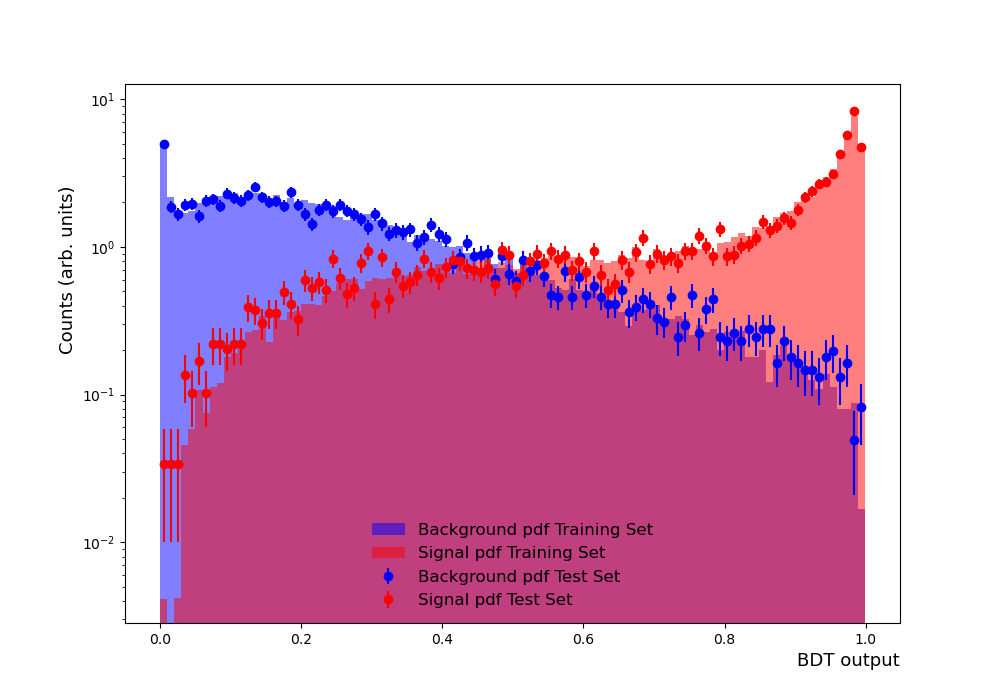
\includegraphics[width=0.6\linewidth]{gallery/results/train_test_without_bkg.png}
    \caption{Example of BDT outputs for training vs. test data. Training data are plotted as shaded histograms and test data are plotted as solid markers, with true background candidates in blue and true signal candidates in red}
    \label{f.ml_bdt_score}
\end{figure}
%
Here, we have essentially distilled all the features of the data into a single variable. Rather than applying cuts by hand on all $m$ features to find the optimal signal-and-background separation (as we would normally do without machine learning), we now only need to apply a one-dimensional cut on the BDT output. When we apply the trained BDT to analyze new data, the model will provide a BDT output for each candidate. We would then choose a BDT threshold value, perhaps $0.5$ for example, then accept all candidates with BDT output $>0.5$ as signal and reject those with BDT output $<0.5$ as background. 

In practice, there often is not a clean separation between the signal and background distributions, as is the case in Fig. \ref{f.ml_bdt_score}, because some features of signal and background candidates can look similar to each other. Due to this overlap, we select the BDT score threshold that best optimizes some metric of interest. In our analyses, the quantity we optimize to is the {\it significance} \cite{BDT},
\begin{equation}
    {\rm Signif} = \frac{N_{\rm sig}}{\sqrt{N_{\rm sig}+N_{\rm bkg}}} \ , \label{eqn.signif}
\end{equation}
where $N_{\rm sig}$ is the number of true signal candidates accepted, $N_{\rm bkg}$ is the number of true background candidates accepted, and $\sqrt{N_{\rm sig}+N_{\rm bkg}}$ represents the statistical uncertainty. Another quantity of interest that represents the effectiveness of classification is the {\it signal-to-background ratio},
\begin{equation}
    {\rm S/B} = \frac{N_{\rm sig}}{N_{\rm bkg}} \ .\label{eqn.s_over_b}
\end{equation}

Another important question to examine in these plots is how much the outputs for training and testing data differ. In the example in Fig. \ref{f.ml_bdt_score}, we observe that the distributions for training data (shaded histograms) and testing data (solid markers) follow each other closely, which means that the BDT outputs are consistent across both datasets. This indicates that the BDT is well-trained and stable. On the other hand, large discrepancies between the training and testing distributions would be a sign of overtraining.

%
\begin{figure}[h!]
    \centering
    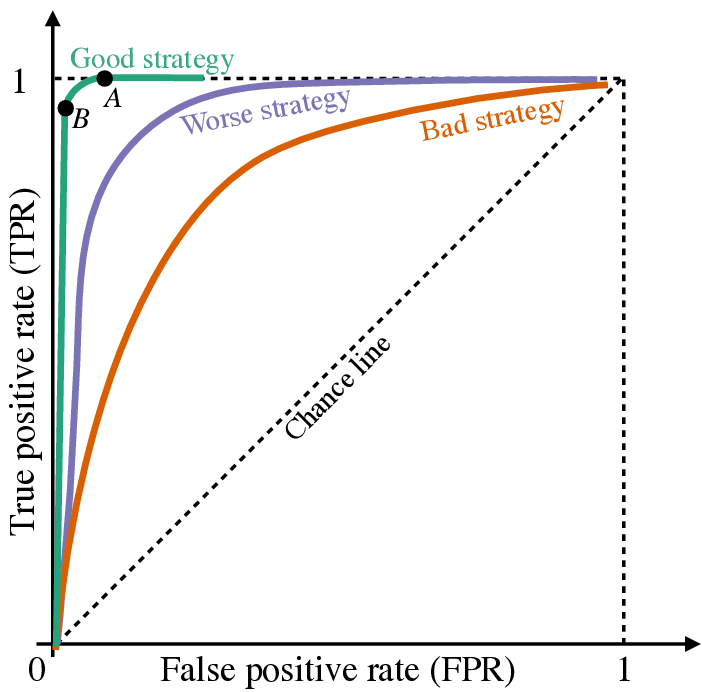
\includegraphics[width=0.5\linewidth]{gallery/ML/roc_ex.png}
    \caption{Examples of receiver operating characteristic (ROC) curves for models with varying levels of performance. Figure from \cite{roc_ex}.}
    \label{f.ml_roc}
\end{figure}
%
Complementary to plots of BDT output, we also examine the {\it receiver operating characteristic} (ROC), shown in Fig. \ref{f.ml_roc}, which illustrates the overall accuracy of the model. On the $y$-axis is the true positive rate (TPR), the fraction of true signal candidates that the model correctly classifies as signal. On the $x$-axis is the false positive rate (FPR), the fraction of true background candidates that the model misclassifies as signal. The ROC curve is produced by calculating the TPR and FPR for various possible threshold values of the BDT output \cite{BDT}, such that each point on the curve represents the result for a different threshold. In this way, the ROC curve summarizes the BDT output distributions of Fig. \ref{f.ml_bdt_score}. (We can separately produce a ROC curve for the testing and training data, which should be very similar to each other for a well-trained model.)

The green ``good strategy" curve in Fig. \ref{f.ml_roc} very closely approximates an ideal model, with a TPR that approaches $1$ very quickly. The dashed ``chance line" denotes the ROC curve resulting from random chance, with the TPR always equal to the FPR. In general, the ROC curve of a properly trained model should be between the good strategy curve and the chance curve, with curves closer to the chance line indicating worse performance. We can also measure the performance more quantitatively by integrating the area under the curve (AUC) from $0$ to $1$ along the $x$-axis. An ideal model would yield ${\rm AUC}=1$, the chance line would yield ${\rm AUC}=0.5$, and as a rule of thumb, a good model should yield ${\rm AUC}>0.8$. 


%-------------------------
\subsection{Examining feature importance with SHAP}
\label{sec.ml_shap}

When using BDTs to analyze data, the choice of features can impact the discriminative ability of the model. Features for which the signal and background distributions look very different will generally provide better discriminative ability than features for which the signal and background are similar. During training, the more discriminative features will have a greater impact on the structure of the BDT.

A method of understanding the relative importance of features used to train a machine learning model is by examining their SHAP values \cite{SHAP}. The SHapley Additive exPlanations (SHAP) tool calculates the marginal contributions of each feature by considering how often a given feature is used during training, and how much each instance of the feature use improves the overall model performance. For BDTs, the SHAP value for each feature is determined by the number nodes in which that feature is used to split the data, as well as the increase in purity resulting from each of those splits.

%
\begin{figure}[h!]
    \centering
    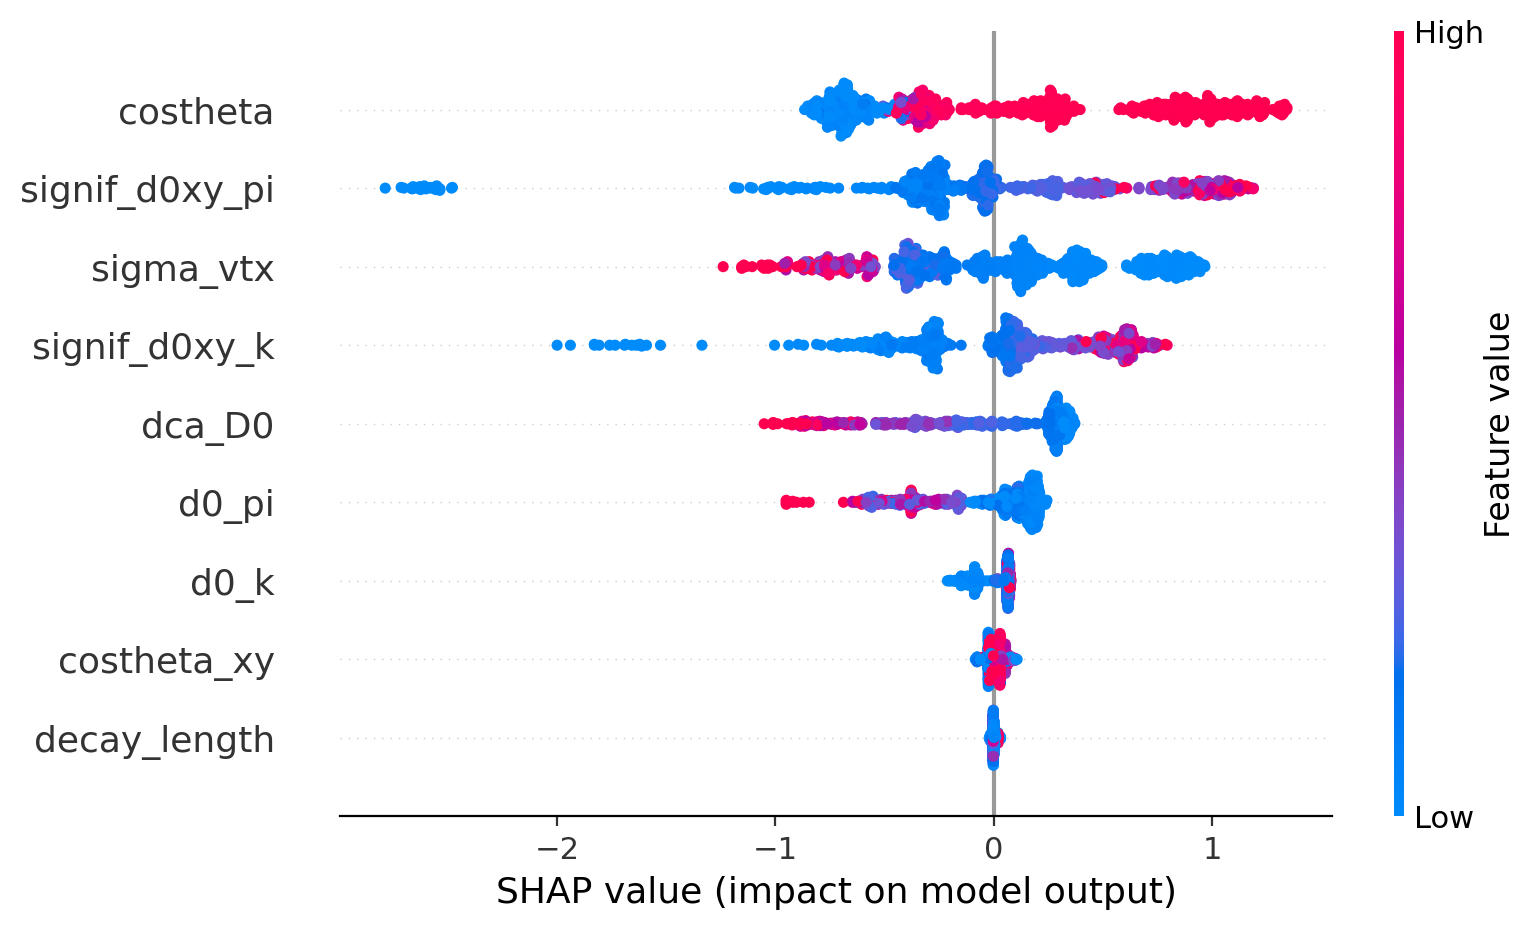
\includegraphics[width=0.95\linewidth]{gallery/ML/ex_shap_beeswarm.png}
    \caption{Example beeswarm plot of SHAP values for topological features used to train a BDT.}
    \label{f.ml_beeswarm}
\end{figure}
%
Fig. \ref{f.ml_beeswarm} shows an example ``beeswarm" plot of the SHAP values for features used to train a particular BDT model. Each point in the plot represents one candidate. Positive SHAP values indicate features that ``push" the BDT output of that candidate toward 1 (signal), and negative SHAP values indicate features that ``push" the BDT output toward 0 (background), with larger absolute values indicating higher impact. The color of each point represents the value of the topological feature for that candidate. The features are organized in order of importance, with the top feature (\texttt{costheta}) being most important. We can see the feature importance reflected in the separation of high value and low value points in the plot. More important features exhibit a more distinct separation of colors, which suggests that these features provide greater discriminative ability.

For example, looking at the \texttt{costheta} feature, we observe that high values of $\cos{\theta}$ (pink) tend to push the BDT outputs of candidates toward 1 while low values tend to push the BDT output toward 0. We can interpret this to mean that candidates with higher (more positive) values of $\cos{\theta}$ are more likely to be signal, and candidates with lower (more negative) values of $\cos{\theta}$ are more likely to be background. If we now look at \texttt{decay\_length}, we observe that neither high and nor low features values push the BDT outputs in a particular direction, so this feature is not very useful in determining whether a given candidate is signal or background.

%
\begin{figure}[h!]
    \centering
    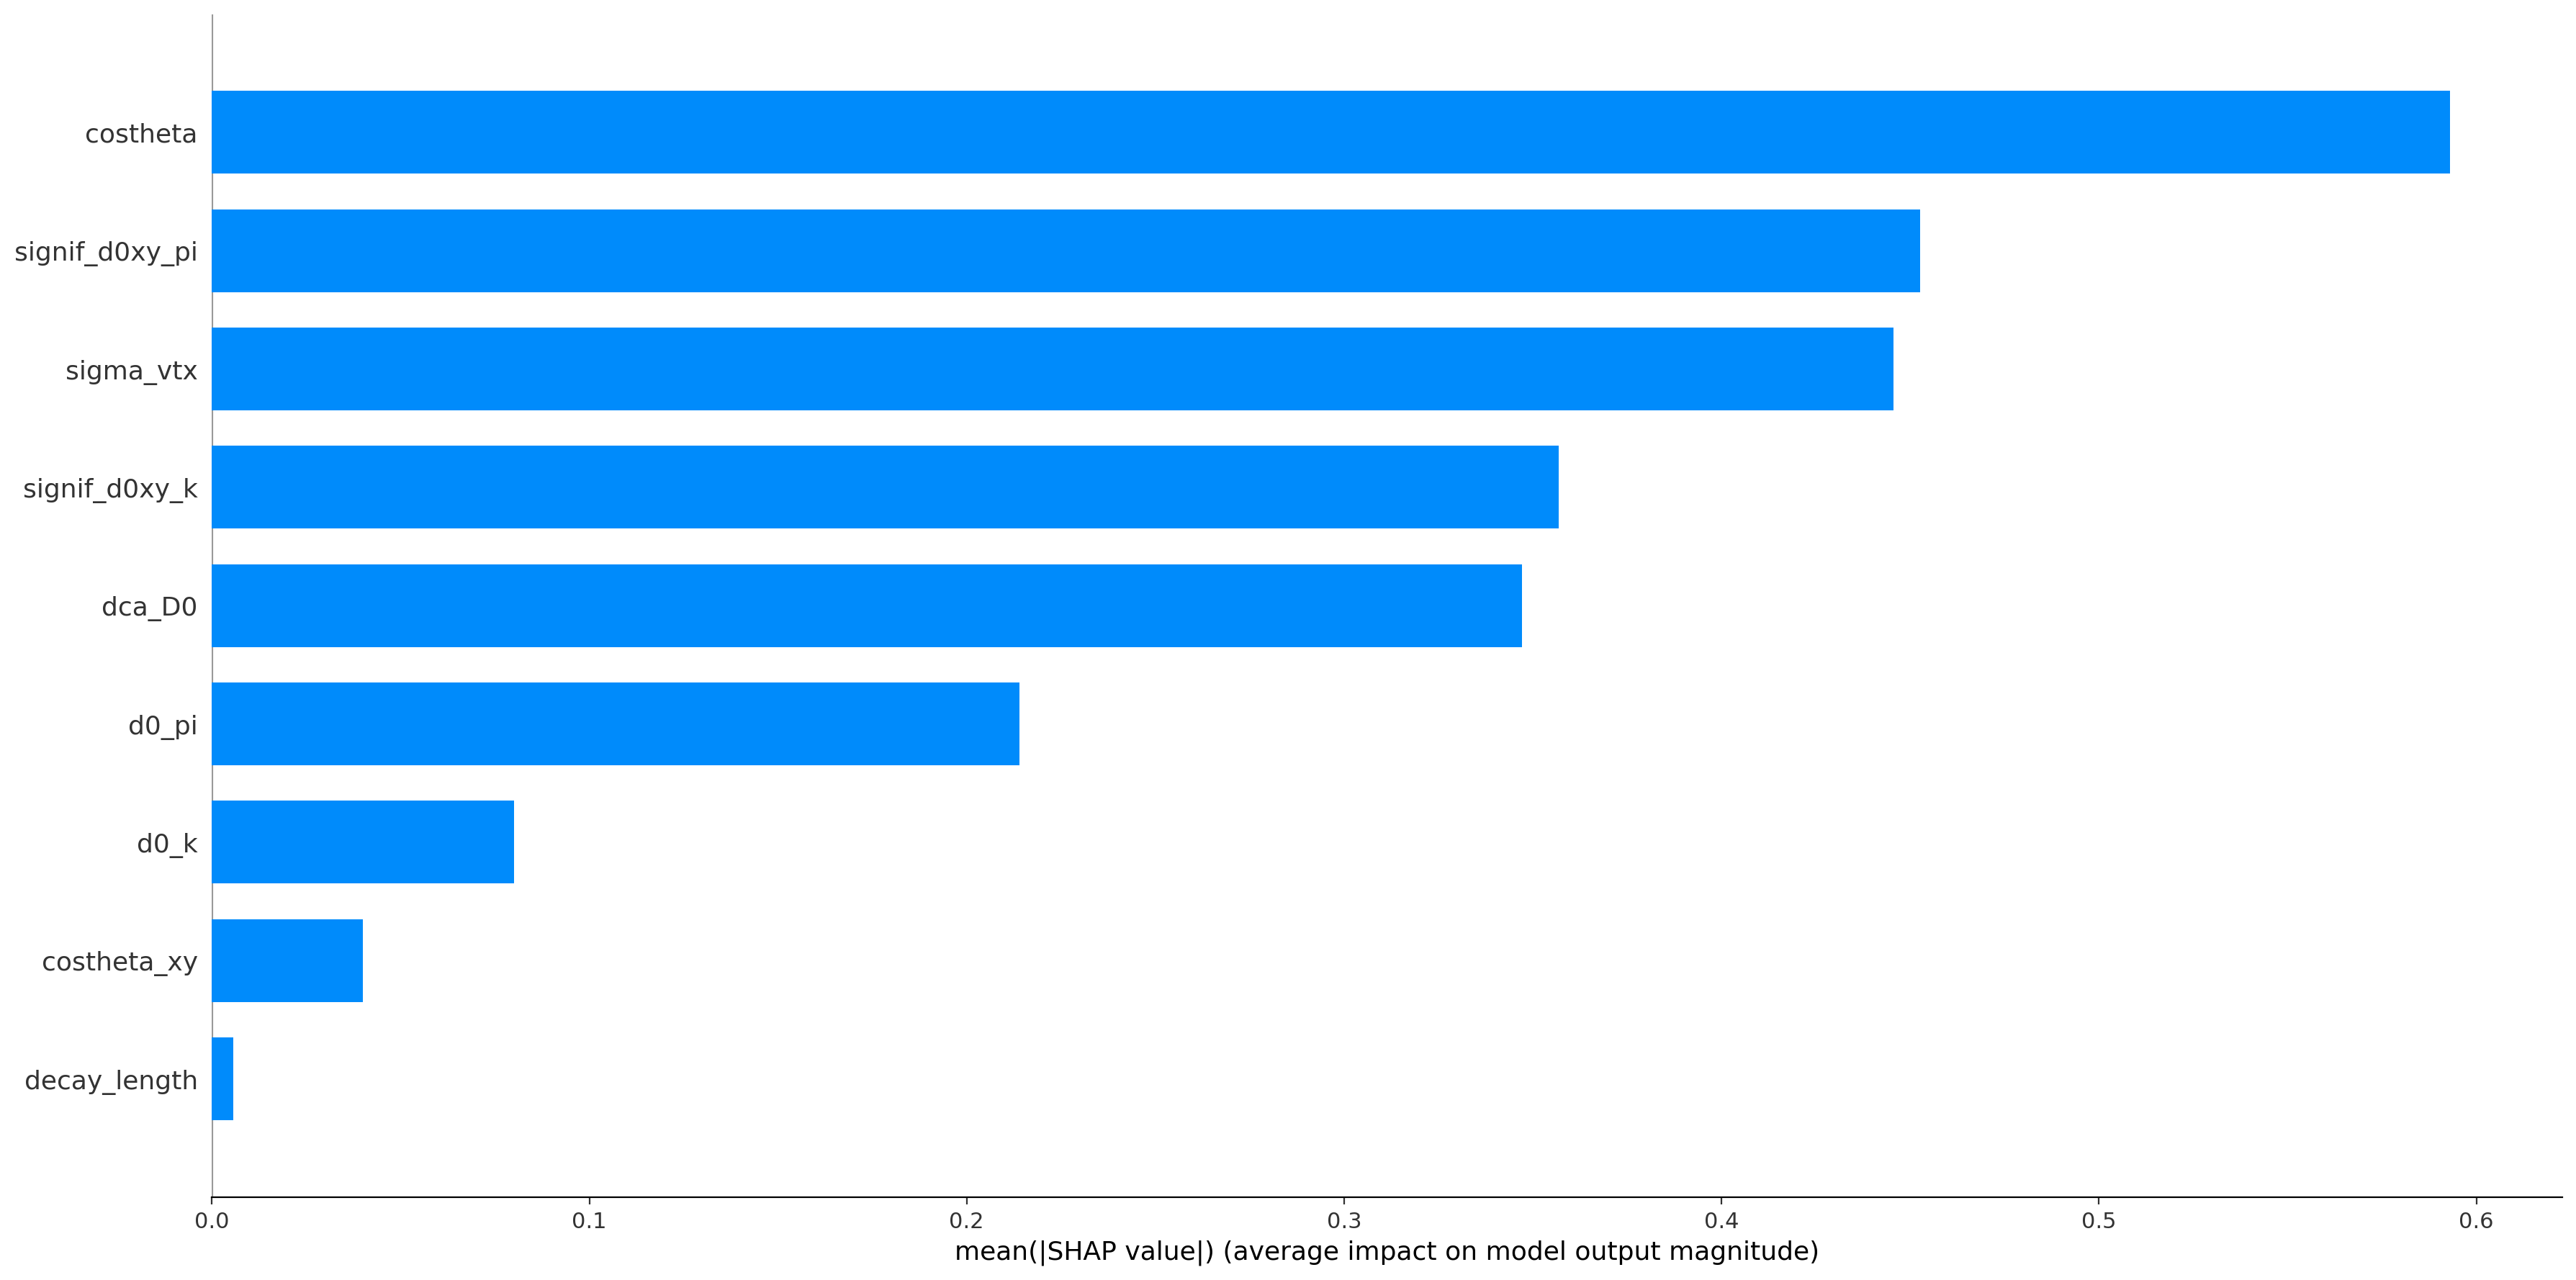
\includegraphics[width=0.95\linewidth]{gallery/ML/ex_shap_feature_impact.png}
    \caption{Example of average SHAP values for topological features used to train a BDT.}
    \label{f.ml_shap}
\end{figure}
%
Fig. \ref{f.ml_shap} summarizes the beeswarm plot by averaging the absolute values of the SHAP results for each candidate. These mean SHAP values provide an overall measure of how much impact each feature has on the BDT outputs, without distinguishing between the particular feature values that push toward signal or background.

%
\begin{figure}[h!]
    \centering
    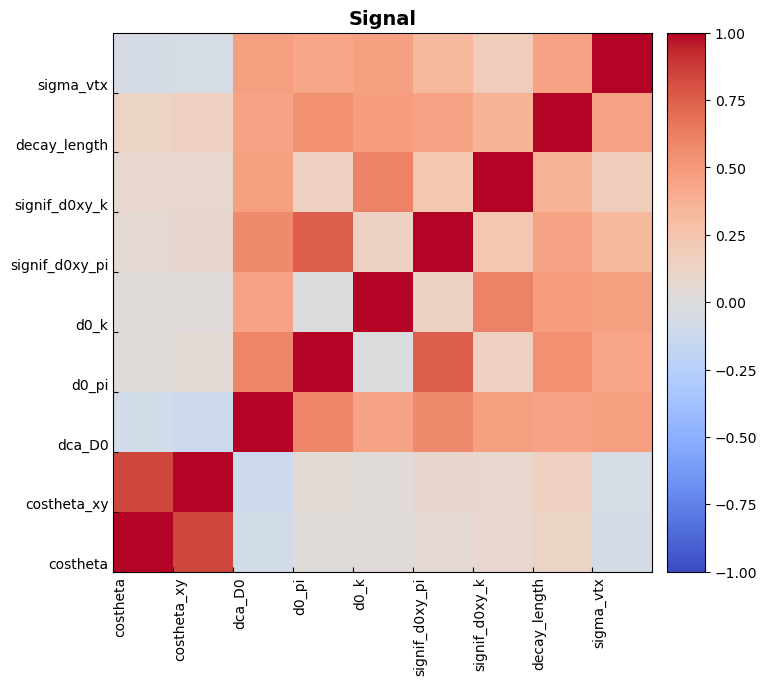
\includegraphics[width=0.7\linewidth]{gallery/ML/ex_correlation_plot_sig.png}
    \caption{Example of feature correlation coefficients. A value of 1 (dark red) indicates perfect positive correlation, and a value of -1 (dark blue) indicates perfect negative correlation.}
    \label{f.ml_corr}
\end{figure}
%
When interpreting SHAP values, it is also important to be cognizant of the correlations between feature values. In Fig. \ref{f.ml_corr}, we plot these feature correlations for the signal candidates. The diagonal entries indicate the correlations of a feature with itself, which are all completely positive as expected. However, we also observe noticeable correlations between different features. In particular, there is very strong positive correlation between \texttt{costheta} and \texttt{costheta\_xy}. This is unsurprising, since $\cos{\theta_{xy}}$ is the component of $\cos{\theta}$ in the $xy$-plane.

Let us now compare the importance of these two correlated features. If $\cos{\theta}$ exhibits very distinct distributions for signal and background candidates and is thus a highly discriminative feature, then we may reasonably expect the same to be true for $\cos{\theta_{xy}}$. However, we notice in Fig. \ref{f.ml_shap} that \texttt{costheta\_xy} has a drastically lower mean SHAP value than \texttt{costheta}. This results from $\cos{\theta_{xy}}$ being very similar to but slightly less discriminative than $\cos{\theta}$, the BDT will tend to cut on $\cos{\theta}$ whenever possible. This leads to $\cos{\theta}$ being rarely used, which artificially suppresses its SHAP value. If we were to train the BDT without including \texttt{costheta}, we would see that \texttt{costheta\_xy} becomes one of the most important features. Thus when features are strongly correlated, their SHAP results should not be taken at face value.

To conclude this section, we note that SHAP is one of many methods that can represent feature importance, and it tends to assign greater importance to features used in the first tree of a BDT, as marginal contributions become increasingly small for trees later on down the boosting chain. Thus, the actual numbers may not be too meaningful, but the plots of SHAP values can nonetheless provide useful qualitative descriptions of how different features impact the model outputs.

%-------------------------
\subsection{Optimizing hyperparameters with Optuna}
\label{sec.ml_optuna}

The final aspect we consider in our analysis is the optimization of hyperparameters, which determine the overall model structure. To determine the most optimal hyperparameter values, we utilize the Optuna package \cite{Optuna}, which tests various points in parameter space and identifies the one which maximizes the ROC AUC of the testing data.

XGBoost provides the following standard BDT hyperparameters \cite{XGBoost_docs}:
\begin{itemize}
    \item \texttt{n\_estimators}: number of trees
    \item \texttt{max\_depth}: maximum depth of each tree
    \item \texttt{learning\_rate} (\texttt{eta}): size of each boosting step
    \item \texttt{min\_child\_weight}: minimum number of candidates in each node
    \item \texttt{min\_split\_loss}: minimum amount of improvement needed to split a node
    \item \texttt{max\_delta\_step}: maximum change in model outputs at each boosting step
    \item \texttt{subsample}: fraction of training data used to train each tree
    \item \texttt{sampling\_method}: algorithm for selecting the subsample for each tree
\end{itemize}
There are also a number of more niche hyperparameters that can be included to adjust the BDT regularization (the conservativeness of the model) and algorithms. For the first three hyperparameters, typical values are on the order of a couple hundred for \texttt{n\_estimators}, 10 or less for \texttt{max\_depth}, and on the order of 0.01 to 0.1 for the \texttt{learning\_rate}. Generally, larger values increase the likelihood of overfitting. By default, values for the other hyperparameters are set such that they provide little to no constraint on the BDT structure. Increasing these values limits the growth or contributions of trees, which is meant to help regularize the model and prevent overfitting.

Although Optuna automates the process of finding the optimal set of hyperparameter values, its results depend on the inputs we provide, such as the combination of hyperparameters we select and the ranges within which we restrict those values.